\documentclass[superscriptaddress, floatfix,nofootinbib,12pt]{revtex4-2}

\usepackage{graphicx}
\usepackage{bm}
\usepackage{dsfont}
\usepackage{amsmath,amsthm,amssymb}
\usepackage[table,xcdraw]{xcolor}

%\usepackage{amsmath,amsthm,amscd,amssymb}
\usepackage[colorlinks=true
,breaklinks=true
,urlcolor=blue
,anchorcolor=blue
,citecolor=blue
,filecolor=blue
,linkcolor=blue
,menucolor=blue
,linktocpage=true]{hyperref}
\hypersetup{
bookmarksopen=true,
bookmarksnumbered=true,
bookmarksopenlevel=10
}
\usepackage[noBBpl,sc]{mathpazo}
\usepackage[papersize={6.7in, 10.0in}, left=.5in, right=.5in, top=1in, bottom=.9in]{geometry}
\linespread{1.05}
\sloppy
\raggedbottom
\pagestyle{plain}

% these include amsmath and that can cause trouble in older docs.
\makeatletter
\@ifpackageloaded{amsmath}{}{\RequirePackage{amsmath}}

\DeclareFontFamily{U}  {cmex}{}
\DeclareSymbolFont{Csymbols}       {U}  {cmex}{m}{n}
\DeclareFontShape{U}{cmex}{m}{n}{
    <-6>  cmex5
   <6-7>  cmex6
   <7-8>  cmex6
   <8-9>  cmex7
   <9-10> cmex8
  <10-12> cmex9
  <12->   cmex10}{}

\def\Set@Mn@Sym#1{\@tempcnta #1\relax}
\def\Next@Mn@Sym{\advance\@tempcnta 1\relax}
\def\Prev@Mn@Sym{\advance\@tempcnta-1\relax}
\def\@Decl@Mn@Sym#1#2#3#4{\DeclareMathSymbol{#2}{#3}{#4}{#1}}
\def\Decl@Mn@Sym#1#2#3{%
  \if\relax\noexpand#1%
    \let#1\undefined
  \fi
  \expandafter\@Decl@Mn@Sym\expandafter{\the\@tempcnta}{#1}{#3}{#2}%
  \Next@Mn@Sym}
\def\Decl@Mn@Alias#1#2#3{\Prev@Mn@Sym\Decl@Mn@Sym{#1}{#2}{#3}}
\let\Decl@Mn@Char\Decl@Mn@Sym
\def\Decl@Mn@Op#1#2#3{\def#1{\DOTSB#3\slimits@}}
\def\Decl@Mn@Int#1#2#3{\def#1{\DOTSI#3\ilimits@}}

\let\sum\undefined
\DeclareMathSymbol{\tsum}{\mathop}{Csymbols}{"50}
\DeclareMathSymbol{\dsum}{\mathop}{Csymbols}{"51}

\Decl@Mn@Op\sum\dsum\tsum

\makeatother

\makeatletter
\@ifpackageloaded{amsmath}{}{\RequirePackage{amsmath}}

\DeclareFontFamily{OMX}{MnSymbolE}{}
\DeclareSymbolFont{largesymbolsX}{OMX}{MnSymbolE}{m}{n}
\DeclareFontShape{OMX}{MnSymbolE}{m}{n}{
    <-6>  MnSymbolE5
   <6-7>  MnSymbolE6
   <7-8>  MnSymbolE7
   <8-9>  MnSymbolE8
   <9-10> MnSymbolE9
  <10-12> MnSymbolE10
  <12->   MnSymbolE12}{}

\DeclareMathSymbol{\downbrace}    {\mathord}{largesymbolsX}{'251}
\DeclareMathSymbol{\downbraceg}   {\mathord}{largesymbolsX}{'252}
\DeclareMathSymbol{\downbracegg}  {\mathord}{largesymbolsX}{'253}
\DeclareMathSymbol{\downbraceggg} {\mathord}{largesymbolsX}{'254}
\DeclareMathSymbol{\downbracegggg}{\mathord}{largesymbolsX}{'255}
\DeclareMathSymbol{\upbrace}      {\mathord}{largesymbolsX}{'256}
\DeclareMathSymbol{\upbraceg}     {\mathord}{largesymbolsX}{'257}
\DeclareMathSymbol{\upbracegg}    {\mathord}{largesymbolsX}{'260}
\DeclareMathSymbol{\upbraceggg}   {\mathord}{largesymbolsX}{'261}
\DeclareMathSymbol{\upbracegggg}  {\mathord}{largesymbolsX}{'262}
\DeclareMathSymbol{\braceld}      {\mathord}{largesymbolsX}{'263}
\DeclareMathSymbol{\bracelu}      {\mathord}{largesymbolsX}{'264}
\DeclareMathSymbol{\bracerd}      {\mathord}{largesymbolsX}{'265}
\DeclareMathSymbol{\braceru}      {\mathord}{largesymbolsX}{'266}
\DeclareMathSymbol{\bracemd}      {\mathord}{largesymbolsX}{'267}
\DeclareMathSymbol{\bracemu}      {\mathord}{largesymbolsX}{'270}
\DeclareMathSymbol{\bracemid}     {\mathord}{largesymbolsX}{'271}

\def\horiz@expandable#1#2#3#4#5#6#7#8{%
  \@mathmeasure\z@#7{#8}%
  \@tempdima=\wd\z@
  \@mathmeasure\z@#7{#1}%
  \ifdim\noexpand\wd\z@>\@tempdima
    $\m@th#7#1$%
  \else
    \@mathmeasure\z@#7{#2}%
    \ifdim\noexpand\wd\z@>\@tempdima
      $\m@th#7#2$%
    \else
      \@mathmeasure\z@#7{#3}%
      \ifdim\noexpand\wd\z@>\@tempdima
        $\m@th#7#3$%
      \else
        \@mathmeasure\z@#7{#4}%
        \ifdim\noexpand\wd\z@>\@tempdima
          $\m@th#7#4$%
        \else
          \@mathmeasure\z@#7{#5}%
          \ifdim\noexpand\wd\z@>\@tempdima
            $\m@th#7#5$%
          \else
           #6#7%
          \fi
        \fi
      \fi
    \fi
  \fi}

\def\overbrace@expandable#1#2#3{\vbox{\m@th\ialign{##\crcr
  #1#2{#3}\crcr\noalign{\kern2\p@\nointerlineskip}%
  $\m@th\hfil#2#3\hfil$\crcr}}}
\def\underbrace@expandable#1#2#3{\vtop{\m@th\ialign{##\crcr
  $\m@th\hfil#2#3\hfil$\crcr
  \noalign{\kern2\p@\nointerlineskip}%
  #1#2{#3}\crcr}}}

\def\overbrace@#1#2#3{\vbox{\m@th\ialign{##\crcr
  #1#2\crcr\noalign{\kern2\p@\nointerlineskip}%
  $\m@th\hfil#2#3\hfil$\crcr}}}
\def\underbrace@#1#2#3{\vtop{\m@th\ialign{##\crcr
  $\m@th\hfil#2#3\hfil$\crcr
  \noalign{\kern2\p@\nointerlineskip}%
  #1#2\crcr}}}

\def\bracefill@#1#2#3#4#5{$\m@th#5#1\leaders\hbox{$#4$}\hfill#2\leaders\hbox{$#4$}\hfill#3$}

\def\downbracefill@{\bracefill@\braceld\bracemd\bracerd\bracemid}
\def\upbracefill@{\bracefill@\bracelu\bracemu\braceru\bracemid}

\DeclareRobustCommand{\downbracefill}{\downbracefill@\textstyle}
\DeclareRobustCommand{\upbracefill}{\upbracefill@\textstyle}

\def\upbrace@expandable{%
  \horiz@expandable
    \upbrace
    \upbraceg
    \upbracegg
    \upbraceggg
    \upbracegggg
    \upbracefill@}
\def\downbrace@expandable{%
  \horiz@expandable
    \downbrace
    \downbraceg
    \downbracegg
    \downbraceggg
    \downbracegggg
    \downbracefill@}

\DeclareRobustCommand{\overbrace}[1]{\mathop{\mathpalette{\overbrace@expandable\downbrace@expandable}{#1}}\limits}
\DeclareRobustCommand{\underbrace}[1]{\mathop{\mathpalette{\underbrace@expandable\upbrace@expandable}{#1}}\limits}

\makeatother


% make sure there is enough TOC for reasonable pdf bookmarks.
\setcounter{tocdepth}{3}

%\usepackage[dotinlabels]{titletoc}
%\titlelabel{{\thetitle}.\quad}
%\usepackage{titletoc}
\usepackage[small]{titlesec}

\titleformat{\section}[block]
  {\fillast\medskip}
  {\bfseries{\thesection. }}
  {1ex minus .1ex}
  {\bfseries}
 
\titleformat*{\subsection}{\itshape}
\titleformat*{\subsubsection}{\itshape}

\setcounter{tocdepth}{2}

\titlecontents{section}
              [2.3em] 
              {\bigskip}
              {{\contentslabel{2.3em}}}
              {\hspace*{-2.3em}}
              {\titlerule*[1pc]{}\contentspage}
              
\titlecontents{subsection}
              [4.7em] 
              {}
              {{\contentslabel{2.3em}}}
              {\hspace*{-2.3em}}
              {\titlerule*[.5pc]{}\contentspage}

% hopefully not used.           
\titlecontents{subsubsection}
              [7.9em]
              {}
              {{\contentslabel{3.3em}}}
              {\hspace*{-3.3em}}
              {\titlerule*[.5pc]{}\contentspage}
%\makeatletter
\renewcommand\tableofcontents{%
    \section*{\contentsname
        \@mkboth{%
           \MakeLowercase\contentsname}{\MakeLowercase\contentsname}}%
    \@starttoc{toc}%
    }
\def\@oddhead{{\scshape\rightmark}\hfil{\small\scshape\thepage}}%
\def\sectionmark#1{%
      \markright{\MakeLowercase{%
        \ifnum \c@secnumdepth >\m@ne
          \thesection\quad
        \fi
        #1}}}
        
\makeatother

\makeatletter

 \def\small{%
  \@setfontsize\small\@xipt{13pt}%
  \abovedisplayskip 8\p@ \@plus3\p@ \@minus6\p@
  \belowdisplayskip \abovedisplayskip
  \abovedisplayshortskip \z@ \@plus3\p@
  \belowdisplayshortskip 6.5\p@ \@plus3.5\p@ \@minus3\p@
  \def\@listi{%
    \leftmargin\leftmargini
    \topsep 9\p@ \@plus3\p@ \@minus5\p@
    \parsep 4.5\p@ \@plus2\p@ \@minus\p@
    \itemsep \parsep
  }%
}%
 \def\footnotesize{%
  \@setfontsize\footnotesize\@xpt{12pt}%
  \abovedisplayskip 10\p@ \@plus2\p@ \@minus5\p@
  \belowdisplayskip \abovedisplayskip
  \abovedisplayshortskip \z@ \@plus3\p@
  \belowdisplayshortskip 6\p@ \@plus3\p@ \@minus3\p@
  \def\@listi{%
    \leftmargin\leftmargini
    \topsep 6\p@ \@plus2\p@ \@minus2\p@
    \parsep 3\p@ \@plus2\p@ \@minus\p@
    \itemsep \parsep
  }%
}%
\def\open@column@one#1{%
 \ltxgrid@info@sw{\class@info{\string\open@column@one\string#1}}{}%
 \unvbox\pagesofar
 \@ifvoid{\footsofar}{}{%
  \insert\footins\bgroup\unvbox\footsofar\egroup
  \penalty\z@
 }%
 \gdef\thepagegrid{one}%
 \global\pagegrid@col#1%
 \global\pagegrid@cur\@ne
 \global\count\footins\@m
 \set@column@hsize\pagegrid@col
 \set@colht
}%

\def\frontmatter@abstractheading{%
\bigskip
 \begingroup
  \centering\large
  \abstractname
  \par\bigskip
 \endgroup
}%

\makeatother

%\DeclareSymbolFont{CMlargesymbols}{OMX}{cmex}{m}{n}
%\DeclareMathSymbol{\sum}{\mathop}{CMlargesymbols}{"50}
\newcommand{\ket}[1]{\left| #1 \right\rangle}
\newcommand{\bra}[1]{\left\langle #1 \right|}
\newcommand{\proj}[1]{\ket{#1}\bra{#1}}
\newcommand{\upket}{\ket{\uparrow}}
\newcommand{\downket}{\ket{\downarrow}}
\newcommand{\braket}[2]{\langle #1|#2 \rangle}
\newcommand{\der}[2]{\frac{\mathrm{d}#1}{\mathrm{d}#2}}
\newcommand{\ketbra}[2]{\left|#1\right\rangle\hskip-1mm\left\langle #2\right|}
\newcommand{\textred}[1]{\textcolor{red}{#1}}

\begin{document}

\title{Wavefunctions can Simultaneously Represent Knowledge and Reality}

\author{Jonte R. Hance}
\email{jonte.hance@bristol.ac.uk}
\affiliation{Quantum Engineering Technology Laboratory, Department of Electrical and Electronic Engineering, University of Bristol, Woodland Road, Bristol, BS8 1UB, UK}
\author{John Rarity}
\affiliation{Quantum Engineering Technology Laboratory, Department of Electrical and Electronic Engineering, University of Bristol, Woodland Road, Bristol, BS8 1UB, UK}
\author{James Ladyman}
\email{james.ladyman@bristol.ac.uk}
\affiliation{Department of Philosophy, University of Bristol, Cotham House, Bristol, BS6 6JL, UK}
\date{16 Jan 2021}

\begin{abstract}

Harrigan and Spekkens give formal definitions for the wavefunction in quantum mechanics to be $\psi$-ontic or $\psi$-epistemic, such that the wavefunction can only be one or the other. We argue that nothing about the informal ideas of epistemic and ontic interpretations rules out wavefunctions representing both reality and knowledge. The implications of the Pusey-Barrett-Rudolph theorem and many other issues need to be rethought in the light of our analysis.

\end{abstract}

\maketitle

\section{Introduction}

Quantum mechanics describes the behaviour of subatomic particles. Unlike classical mechanics, where particles are attributed particular values of position and momentum, quantum mechanics attributes wavefunctions, which give probability amplitudes for possible values of position, momentum and other observables. The products of the standard deviation of position and the momentum (and other pairs of incompatible observables) have a minimum value given by the uncertainty principle \cite{Kennard1927Quantenmechanik}, but otherwise the situation seems similar to how a probability distribution is used to represent incomplete knowledge of a state. For example, probability functions in classical statistical mechanics are used because, while we do not know the exact state of all the particles in a gas, we do know a lot about them on average --- these probability distributions reflect knowledge about the distribution of particles over microstates. So, perhaps the wavefunction in quantum mechanics represents knowledge about quantum particles (is epistemic) and does not represent the real state of particles (is not ontic).

A very influential paper by Harrigan and Spekkens gives formal definitions for the wavefunction being $\psi$-ontic or $\psi$-epistemic, such that the wavefunction can only be one or the other \cite{Harrigan2010Nonlocality}. On the contrary, we argue that nothing about the informal ideas of epistemic and ontic interpretations or states rules out wavefunctions representing both reality and knowledge. If this is right then the now standard definitions create a false dichotomy. There are interpretations that are intended to be exclusively epistemic, such as Fuch's Quantum Bayesianism (QBism), which treat the wavefunction as representing knowledge about possible results, rather than a physical state of the world \cite{Fuchs2002Info,Fuchs2014QBism}, or exclusively ontic, such as dynamical collapse theories \cite{Penrose1996Gravity, Ghirardi1986Unified}), Bohmian mechanics \cite{Bohm1952Suggested} and Everett's relative-state interpretation \cite{Everett1957Relative}, which take the wavefunction to represent something physical. However, this is no reason to define epistemic and ontic interpretations exclusively, because the informal ideas do not exclude each other, as the next section shows. The following sections explain Harrigan and Spekkens's formalisation, and show how their definitions of $\psi$-ontology and $\psi$-epistemicism simply presuppose that the wavefunction cannot represent both knowledge and reality.

\section{Ontic and Epistemic Interpretations of Terms in Physical Theories}

Wavefunctions, like particle coordinates or vector fields, are part of the mathematical apparatus of physical theory. Such a term in physical theory has an ontic interpretation (is an `ontic state') when it is taken to represent how the world is independently of our knowledge of it \emph{to some extent or other}.\footnote{The terminology of 'ontic' versus 'epistemic' states is problematic not only for the reasons we give, but it has become standard among physicists working in quantum foundations.} For example, the number 9.81 represents the acceleration due to gravity near the surface of the Earth. It is not perfectly accurate and depends on the conventional choice of units, but arguably all representations are like this to some extent. Many mathematical terms used in classical physics, whether scalars, like mass or charge, or vectors, such as magnetic field strength or linear momentum, are apt to be taken as representing real physical properties.\footnote{Note that this is not to say that wavefunctions are physical things, but that they represent something physical, just as the correspondence between your fingers and the numbers one to ten does not make the numbers themselves physical \cite{Wallace2010StateRealism,Schlosshauer2012Implications,Hermens2021Howreal}.}

In his influential review of the PBR theorem, Matt Leifer says that an ontic state represents `something that objectively exists in the world, independently of any observer or agent' \cite{Leifer2014Review}. This is stronger than the definition above because it rules out that the term also represents our knowledge of the world as well. He gives the example of the ontic state of a single classical particle being its position and momentum.\footnote{Leifer's corresponding example of an epistemic state is then the probability distribution over the particle's phase space.}

On the other hand, a term in physical theory has an epistemic interpretation (is an `epistemic state') when it is taken to represent knowledge of the world \emph{to some extent or other}. This seems a reasonable response to the peculiarity of quantum mechanics --- phenomena such as contextuality, entanglement and collapse could involve incomplete knowledge and Bayesian updating of assigned probabilities. This has led to interpretations of the wavefunction as representing \emph{only} knowledge (as in QBism, and also Ben-Menahem's interpretation of ``quantum probabilities as objective constraints on the information made available by measurement" \cite{Benmenahem2017PBR}).

Simon Friedrich says a ($\psi$-)epistemic interpretation is any view according to which ``quantum states do not represent features of physical reality, but reflect, in some way to be specified, the epistemic relations of the agents who assign them to systems they are assigned to'' \cite{friederich2014Interpreting}. So he (and Leifer) agree that epistemic and ontic interpretations are exclusive of each other, so that an epistemic interpretation of a term rules out that the term represents the world as well (and this is so for Harrigan and Spekkens too as explained in the next section). On the other hand, our definitions do not make them exclusive of each other (and the positive second part of Friederich's definition of a ($\psi$-)epistemic interpretation is very similar to our definition of one).

In the case Leifer considers there is clearly a many-one map between the epistemic state and the ontic state, in the sense that many epistemic states are compatible with the true state of the system (because there are many probability distributions that give a non-zero probability to a given state of the particle). 

However, this is not so for the ontic state. Only one mathematical representation is compatible with the underlying state of the system, because the mathematical representation of each possible microstate is a complete specification of all the degrees of freedom of the system over which the probability distribution is defined. As the next section explains, Harrigan and Spekkens make this difference between a many-one and one-one mapping definitive of epistemic and ontic interpretations.

Not everything in physics is as straightforward as the toy model Leifer considers, and it is not always clear whether terms in physical theories represent real things (for example, component versus resultant forces, gauge etc.). In quantum mechanics individual particles do not in general have their own pure quantum states. Nothing about the idea of a determinate reality requires that all physical states are decomposable into the states of particles, and the states of quantum field theory do not take individual particles to be the fundamental bearers of physical properties. The probability distributions we get from quantum mechanics are over eigenvalues associated with observables, not over underlying states-of-the-world as in classical statistical mechanics. For all these reasons and more the framework and definitions of the next section that have become orthodox are questionable.

\section{The Ontological Models Framework}

\begin{figure}
    \centering
    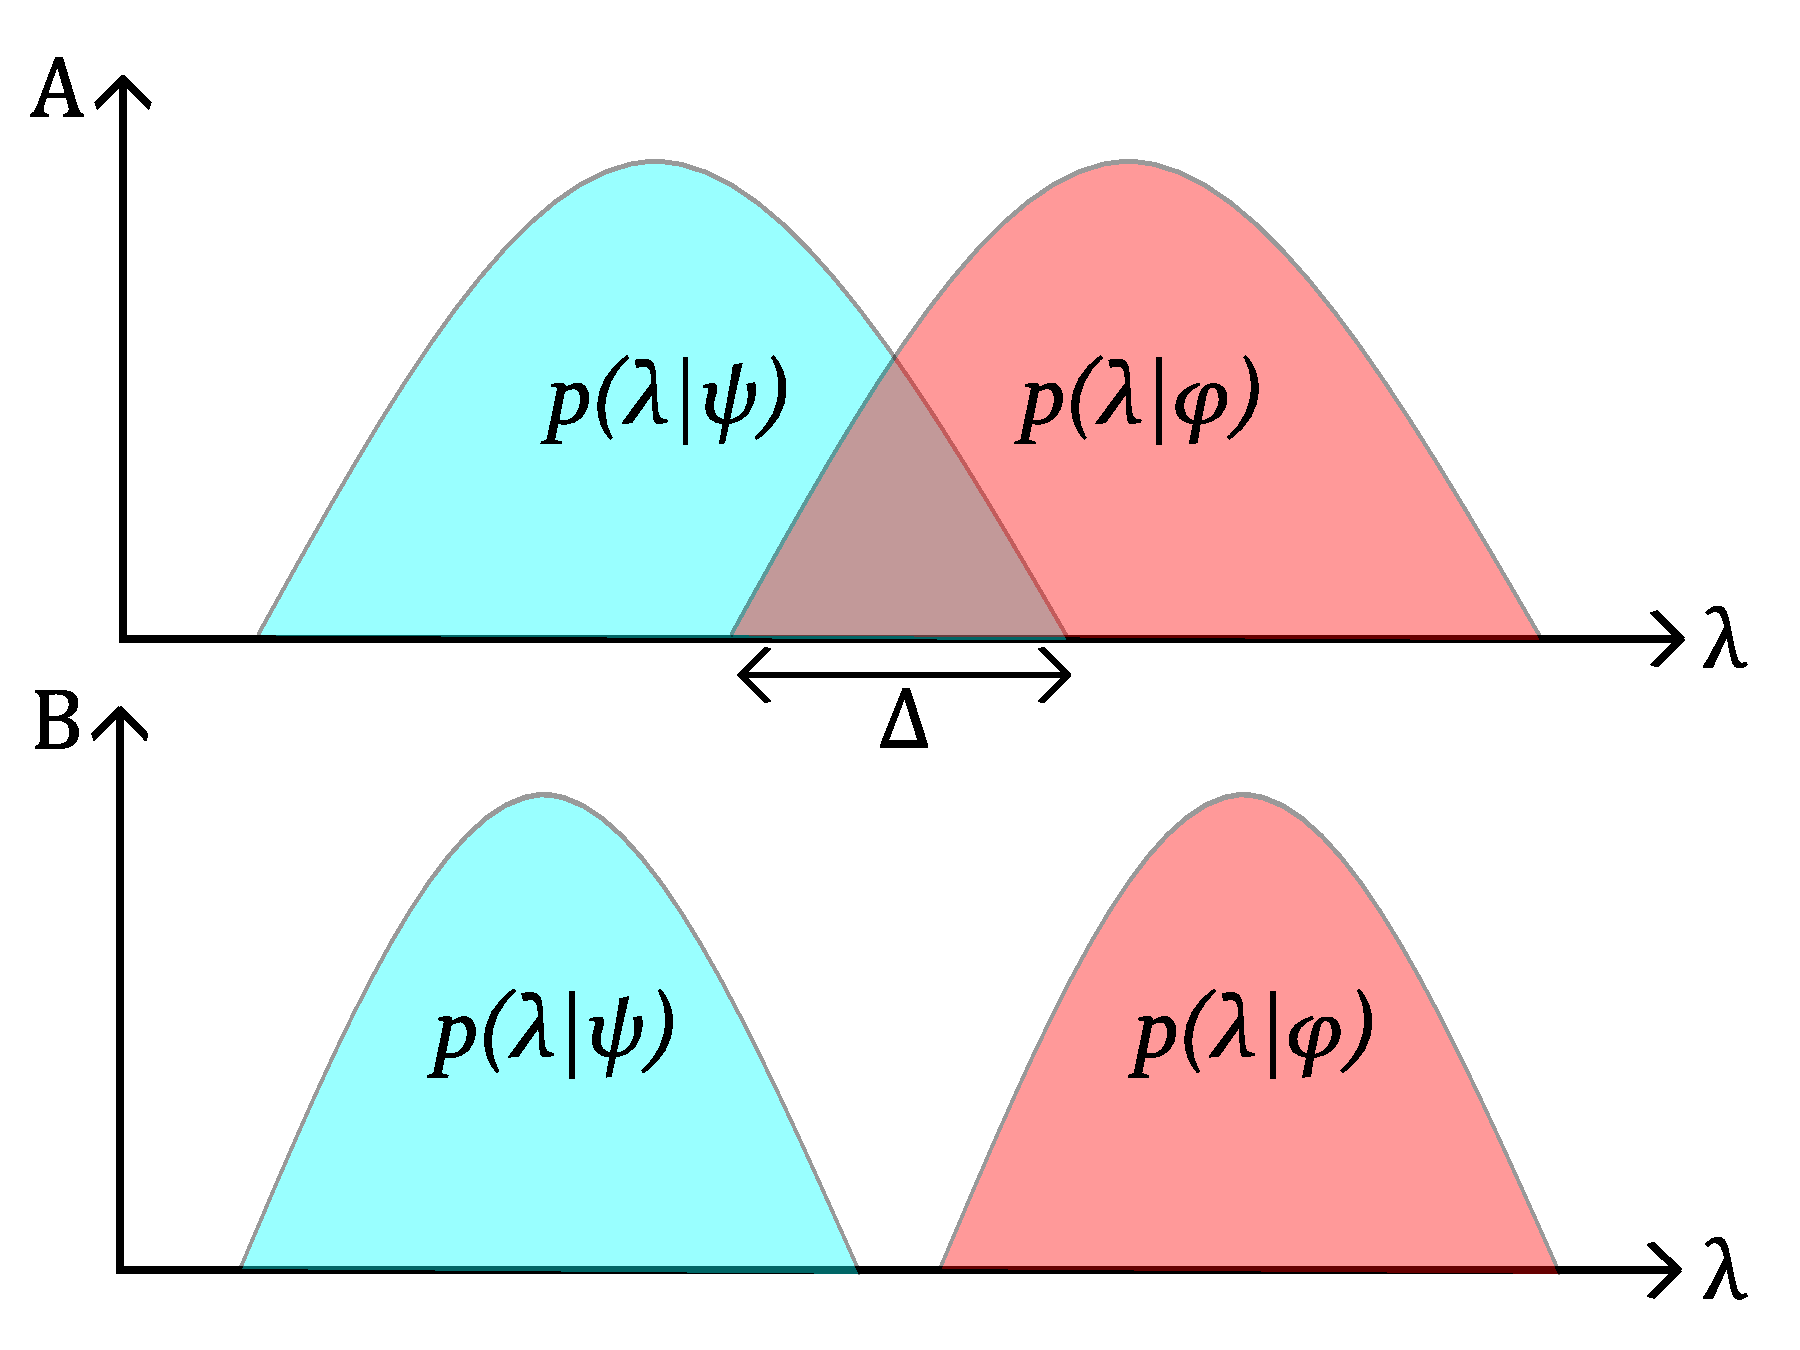
\includegraphics[width=\linewidth]{StateOverlapDiag.pdf}
    \caption{Harrigan and Spekkens's $\psi$-epistemic (A) and $\psi$-ontic (B) models of reality. Wavefunctions $\psi$ and $\varphi$ each have probability distributions over state-space $\Lambda=\{\lambda\}$. In a $\psi$-epistemic model, these can overlap over a subspace \textit{$\Delta$}, so a state $\lambda$ within this overlap could be represented by both $\psi$ and $\varphi$. However, in their formalism, in $\psi$-ontic models, each state can only be represented by one wavefunction.}
    \label{fig:Graphs}
\end{figure}

Harrigan and Spekkens's Ontological Models framework considers how the wavefunction $\psi$ relates to some particular underlying real state of the world $\lambda$, from the space $\Lambda$ of possible such states \cite{Spekkens2005Contextuality,Rudolph2006Ontological,Harrigan2007Ontological,Spekkens2007EpistTot, Harrigan2010Nonlocality}. So understood the wavefunction gives the relative (Born) probability $p^\psi_A(S)$ that, upon measurement, a certain degree of freedom (described by observable $A$) will have the specific value $S$ (or range of values). It can be represented as a normalised vector $\ket{\psi}$ in a Hilbert Space $\mathcal{H}$, where there is a complete orthonormal basis of vectors, corresponding to possible values of $A$ (with one or more vectors per value, e.g. $\ket{S}$ for $S$).

In any hidden variable model, each observable $A$ has an associated response function $\mathcal{A}(S\vert\lambda)$, which gives the probability for state $\lambda$ that a measurement of variable $A$ would give an outcome in set $S$ \cite{Schlosshauer2012Implications}. There is also $p(\lambda\vert\psi)$, the probability a situation described by wavefunction $\psi$ is in a given state $\lambda$ (normalised over $\psi$'s support in state space $\Lambda_\psi$).\footnote{The 'support' of a probability distribution is the set of all the values to which it assigns a non-zero probability.} The framework assumes both of these are probabilities (meaning both must be non-negative and additive) rather than quasiprobabilities \cite{Harrigan2007ProbDistn}.\footnote{Note, Harrigan and Rudolph extend this framework further by including a treatment of preparation and measurement devices.}
This requires,
\begin{equation}
    p^\psi_A(S)
    =\vert\braket{S}{\psi}\vert^2
    = \int_{\Lambda}\mathcal{A}(S\vert\lambda) p(\lambda\vert\psi) d\lambda
\end{equation}

Imagining our (arbitrary) observable $A$ had the original wavefunction $\ket{\psi}$ as a possible state after measurement (i.e. $\ket{S}=\ket{\psi}$), we find (as $\vert\braket{\psi}{\psi}\vert^2=1$, and $p(\lambda\vert\psi)$ is normalised over $\Lambda_\psi$ \cite{Maroney2012Statistical})
\begin{equation}
    \forall\lambda\in\Lambda_\psi,\;\mathcal{A}(\psi\vert\lambda) = 1 
\end{equation}

If we now imagine a second possible wavefunction, $\varphi$, with its own probability distribution $p(\lambda\vert\varphi)$ over support $\Lambda_\varphi$, obeying these same rules, we see
\begin{equation}
    \vert\braket{\psi}{\varphi}\vert^2
    = \int_{\Lambda}\mathcal{A}(\psi\vert\lambda) p(\lambda\vert\varphi) d\lambda
\end{equation}

By restricting this to the subspace $\Lambda_\psi$, we define
\begin{equation}
\begin{split}
\Delta&\equiv\int_{\Lambda_\psi}\mathcal{A}(\psi\vert\lambda) p(\lambda\vert\varphi) d\lambda\\
    &=\int_{\Lambda_\psi} p(\lambda\vert\varphi) d\lambda\leq\vert\braket{\psi}{\varphi}\vert^2
    \end{split}
\end{equation}

If $\Delta>0$, this overlap of $p(\lambda\vert\varphi)$ and $\Lambda_\psi$ is taken to imply that the two wavefunctions in this model are epistemic states, because the same underlying state $\lambda$ could be represented by either depending on what it known about the system.\footnote{However, note, this doesn't mean that they necessarily represent the underlying state equally well --- for a given $\lambda$ in this overlap, $p(\lambda\vert\psi)$ needn't equal $p(\lambda\vert\varphi)$.} Harrigan and Spekkens take the existence of two distinct wavefunctions with overlapping support within a model as necessary and sufficient for that model being $\psi$-epistemic (and not $\psi$-ontic). The idea is that, since the wavefunction is not determined by the underlying state, so that two different wavefunctions can represent it, some other factor must fix the wavefunction, and that factor is what is known about the system.

Harrigan and Spekkens claim all models that don't meet their criterion for being $\psi$-epistemic are $\psi$-ontic, based on how, classically, states can be either ontic (points on state space) or epistemic (probability distributions on state space) as discussed above.\footnote{Schlosshauer and Fine apply the terms Mixed and Segregated to these quantum models, rather than $\psi$-epistemic and $\psi$-ontic \cite{Schlosshauer2012Implications}, which better characterises the divide in wavefunction overlap.}

Harrigan and Spekkens give three subcategories of $\psi$-ontology. In the strongest (the $\psi$-complete model), the wavefunction describes the system's state completely and no hidden variables are left out by it (as in Everettian interpretations). In the other two models, both referred to as $\psi$-supplemented, the state is supplemented by some hidden variable --- in the first as a one-to-one mapping between the wavefunction and the state; and in the second where wavefunctions can map to more than one state (but each state still only maps to one wavefunction). While the wavefunction may not itself be the state, in this framework, $\psi$-ontic models have each state correspond to at most one wavefunction (see Fig. \ref{fig:Graphs}B), meaning all wavefunctions have disjoint support in the state-space:
\begin{equation}
    \forall\psi,\varphi,\;s.t.\psi\neq\varphi;\;\Lambda_{\psi}\cap\Lambda_{\varphi}=\oslash
\end{equation}

\section{Analysing Harrigan and Spekkens's Definitions}

In Harrigan and Spekkens's framework, only $\psi$-epistemic models allow multiple wavefunctions to overlap on the same underlying real state of the world (see Fig. \ref{fig:Graphs}A). Although, given the assumptions of the Ontological Models formalism, this is a sufficient condition for a model being interpreted epistemically, it is not a necessary one, because it is possible that knowledge is included in the wavefunction but this one-to-one mapping still holds (i.e. $\Delta=0$) --- an epistemic model without wavefunction overlap on state space.

An even broader condition would be that it is sufficient for a model to be interpreted epistemically when the response functions for individual $\lambda$ within a wavefunction's support $\Lambda_\psi$ for a given variable $A$, aren't equal to the Born probability for the wavefunction for that variable:
\begin{equation}
\begin{split}
  \exists\{\psi,S,A\},\;s.t.\;\neg((\mathcal{A}(S\vert\lambda)=p^\psi_A(S)\;\forall\lambda\in\Lambda_{\psi})\\
  \implies\;\psi\text{-epistemic}
  \end{split}
\end{equation}
This condition implies the Born probability is just the weighted average of response functions over $\Lambda_\psi$, rather than directly related to the specific $\lambda$ representing the actual state of the world. All cases of overlap obey this condition, as within $\Lambda_\psi$, $\mathcal{A}(\psi\vert\lambda)=1$, but $p^\varphi_A(\psi)=\vert\braket{\psi}{\varphi}\vert^2$ which isn't equal to 1 if $\psi\neq\varphi$. However, we can also imagine cases without overlap obeying this condition for an epistemic interpretation, as it applies to the response function of any variable, rather than one giving a final result of measurement of a system attributed the state $\psi$ whatever that is.

Harrigan and Spekkens's criterion for a model being $\psi$-ontic --- that wavefunctions never have overlapping support in the space of undelying states --- assumes it cannot also be $\psi$-epistemic by definition.

$\psi$-ontic models, in their formalism, either take the wavefunction to be the exact underlying state, or as representing some reduced-information element of the state. What they ignore is that this reduced-information representation might need to be supplemented to get anything usable as a wavefunction. This would imply a wavefunction could represent an element of reality at its core, but also vary depending on additional factors --- such as the knowledge of the observer. The wavefunction could represent both a part of the underlying state of the world, and an observer's knowledge of it. Wavefunctions representing different elements of reality could still be disjoint, but, because of the supplementing factor (e.g. differing knowledge), wouldn't have to be.

Even assuming the Ontological Models Framework, our above definition for an ontic interpretation of $\psi$ just requires that the Born probability $p^\psi_A(S)$ depends somewhat on the underlying state $\lambda$. The only time this is not the case is when any overlap of wavefunctions in state space entirely corresponds to the inner product of those wavefunctions --- therefore
\begin{equation}
\begin{split}
    \neg(\Delta(\psi,\varphi)=\vert\braket{\psi}{\varphi}\vert^2,\;\forall\psi,\varphi)\\
    \implies\psi\text{-ontic}
    \end{split}
\end{equation}

Leifer and Maroney, and separately Ballentine, have proven that the only time this isn't the case (when $\Delta(\psi,\varphi)=\vert\braket{\psi}{\varphi}\vert^2,\;\forall\psi,\varphi$) violates the Kochen-Specker Theorem \cite{Leifer2013MaxEpist,Ballentine2014Ontological} \footnote{Maroney refers to models where $\Delta$ is always 0 as maximally $\psi$-ontic and where $\Delta$ is always $\vert\braket{\varphi}{\psi}\vert^2$ as maximally $\psi$-epistemic, but says nothing about a general condition for a model being $\psi$-ontic \cite{Maroney2012Statistical}.}.

Since $p^\psi_A(S)$ depending on $\lambda$ ($\Delta$ not having to equal $\vert\braket{\psi}{\varphi}\vert^2,\;\forall\psi,\varphi$) doesn't necessarily imply it is entirely determined by $\lambda$ ($\Delta$ being 0 $\forall\psi,\varphi$), it can meet the conditions for being both ontic and epistemic.

Harrigan and Spekkens admit that all models that aren't $\psi$-complete could be said to have an epistemic character, especially where multiple states map onto one wavefunction, given that this associates the wavefunction with a probability distribution over state space. However, they say they are instead interested only in pure quantum states --- hence their definitions being based on overlap, given they claim, with pure states, ``$\psi$ has an ontic character if and only if a variation of $\psi$ implies a variation of reality and an epistemic character if and only if a variation of $\psi$ does not necessarily imply a variation of reality" \cite{Harrigan2010Nonlocality}. Hardy agrees, saying, given no overlap between the support of wavefunctions on the underlying state, we could deduce the wavefunction from $\lambda$, which he takes to mean the wavefunction would be written into the underlying reality of the world \cite{Hardy2013QStatesReal}. However, this is questionable, given, as we said earlier, that correlation between $\lambda$ and a wavefunction doesn't necessarily make that wavefunction physical, any more than the correspondence between your fingers and the numbers 1-10 makes those numbers physical \cite{Schlosshauer2012Implications} (which is why we earlier defined wavefunction-ontic as the wavefunction representing the real state, rather than being real itself).

Further, considering the wavefunction to be ontic if and only if variation in it implies variation in the underlying state ignores the fact that while ontic models require that the wavefunction represent an element of reality, they need not represent {\it only} such an element. Even for pure states, so long as we are not considering a $\psi$-complete model, there is always some factor supplementing the wavefunction in the full underlying state of the world --- so, conversely, knowledge could supplement that representation of reality to give us the wavefunction. Therefore, there is no reason for change in wavefunction to imply change in reality in an ontic model, even for pure states.

This is demonstrated by $\psi$-dependent models \cite{Schlosshauer2012Implications}. In a $\psi$-dependent model, the response functions depend on $\psi$ --- individual overlap possibilities for each possible state are given by the relevant measurement probabilities --- rather than being uniform. The simplest case of this is when $p_\psi$ is uniform across $\Lambda_\psi$, as, to retrieve the Born probabilities, $\mathcal{A}^\psi(S,\lambda)$ must then depend on $\psi$. As the wavefunction still to some degree reflects the underlying state, these models are ontic in our sense. However, they also allow overlap of wavefunctions on state space, making them $\psi$-epistemic --- Schlosshauer and Fine give an ontic model which is also $\psi$-epistemic, also showing models can be both.

\section{Consequences}

In the light of the above we can create wavefunction-epistemic models of the wavefunction which circumvent no-go arguments typically applied to wavefunctions being epistemic --- such as the Pusey-Barrett-Rudolph (PBR) argument.

Pusey et al showed, given certain assumptions, that any model that is $\psi$-epistemic by Harrigan and Spekkens's criterion (i.e. allows wavefunction-overlap on state space) always contradicts quantum theory \cite{Pusey2012OnTheReality}. However, these assumptions (as given by Leifer \cite{Leifer2014Review}) assume the definition of $\psi$-epistemic as the wavefunction only representing knowledge about an underlying state.\footnote{The key assumption of Pusey et al's argument, and other no-go theorems aiming to prove the incompatibility of $\psi$-epistemic models with quantum physics, is referred to as Preparation Independence Postulate (PIP). This assumes that any two systems prepared separately can be assumed not to have elements of their underlying states correlated (that two separate states together can just be represented by their tensor product). This is not a trivial assumption \cite{Lewis2012Compatible} --- it does not just rule out superdeterminism (non-causal correlations), but any correlation between two separately-prepared subsystems. Given the underlying state posited by the ontological models framework is that of the world, rather than that of any individual system, and subsystems often have hidden correlations (off-diagonal density-matrix terms) in quantum mechanics, we cannot arbitrarily say the extent to which any two real systems are separable.}

By taking the wavefunction to also represent elements of reality, we can circumvent the PBR argument, while still allowing overlap. For instance, we can do this by creating models of the wavefunction like Schlosshauer and Fine's, where, due to $\psi$-dependence, overlap between wavefunctions on state space can exist, but be set to go to 0 when wavefunctions are orthogonal, avoiding PBR-contradiction.

Alongside this, our sufficient condition for models being epistemic doesn't require these models to allow wavefunction overlap on state space. This means, even if these assumptions are valid, and so wavefunction overlap is incompatible with quantum physics, it wouldn't necessarily affect all epistemic models.

On our view, the wavefunction can represent both elements of reality as it is independently of us, and elements of our knowledge of it. The PBR argument only rules out models that have require both wavefunction overlap on state space, and assumptions related to the wavefunction solely representing knowledge. The same applies for other no-go theorems based on these definitions, such as Colbeck and Renner's \cite{Colbeck2012Correspondence}, Patra et al's \cite{Patra2013NoGo}, Hardy's \cite{Hardy2013QStatesReal}, and Ruebeck et al's \cite{Ruebeck2020Epistemic}.

\section{Conclusion}

Even in the ontological models framework, models can be simultaneously ontic and epistemic --- the wavefunction can represent both elements of reality, and elements of an observer's knowledge about that reality. Harrigan's and Spekkens's terms, $\psi$-ontic and $\psi$-epistemic, do not formalise the informal ideas correctly. In light of the above analysis, all current no-go theorems for the wavefunction representing knowledge (such as the PBR theorem, Colbeck and Renner's, Hardy's, Patra et al's, and Ruebeck  et al's) actually at best only rule out wavefunction overlap, and not the wavefunction representing knowledge as is usually claimed.

\begin{acknowledgements} \textit{Acknowledgements:} We thank Hatim Salih and Karim Thebault for useful discussions. This work was supported by the University of York's EPSRC DTP grant EP/R513386/1, and the Quantum Communications Hub funded by the EPSRC grant EP/M013472/1.\\
\textit{Author Contribution Statement (CRediT):} JRH --- Conceptualisation, Methodology, Writing (Original Draft), Visualisation; JR --- Supervision, Writing (Review and Editing), Funding acquisition; JL --- Conceptualisation, Methodology, Writing (Review and Editing), Supervision\\
\textit{Competing Interest Statement:} The authors declare that there are no competing interests.
\end{acknowledgements}

\bibliographystyle{apsrev4-2}
\bibliography{ref.bib}

\appendix
\section{Appendix --- Analogous Concepts}
The thermodynamic entropy $S$ of a system is also a candidate for being both ontic and epistemic. The entropy assigned to a system depends on knowledge of it. For instance, the entropy assigned to an equally divided box of particles is higher if an observer can distinguish these particles than if they cannot \cite{Cheng2009Thermodynamics}. However, that doesn't mean either that one entropy is correct and the other is not, nor that they are both solely expressions of knowledge and so equally `correct' (as would be analogous to Harrigan's and Spekkens's definitions of $\psi$-ontology and $\psi$-epistemicism respectively). Instead, both represent the system as it is independently of us to some extent, while also representing what is known about it \cite{Ladyman2008UseofITEntropy}.

While the ontological models framework considers pure, rather than mixed states, the latter also seem to represent both the underlying state of a system and knowledge of it, to produce overlapping states in the theory for the same real state of the world. An example of this is the singlet state of spin. If we trace out one subsystem to consider the other, lack of knowledge about the other subsystem makes the state of each maximally mixed in every basis, and there is no possible pure state about which we could be ignorant (because there is no pure state of one particle's spin which is empirically equivalent to the maximally mixed state of spin in every basis). Despite this, something about the world independently of what we know about is represented by the maximally mixed state because it gives the correct relative frequencies for measurements on just one particle.\footnote{Similarly, if we believe a state is an equal mix of $\upket_x$ and $\downket_x$, but it is actually the pure state $\upket_z$, neither the mixed or pure state would wrongly describe the results of an $x$-measurement: they would just reflect differing knowledge of the system.} Caves et al give an account where it is consistent for different observers to believe a situation represented by different states, but for all observers to believe the state pure (though this is for a situation where no underlying real state is assumed) \cite{Caves2002conditions}.

\section{Appendix --- Issues with an Assumed Underlying State \texorpdfstring{$\lambda$}{lambda}}
As mentioned above, there are a number of issues with the idea of an underlying state assumed by the Ontological Models Framework. Classically, points in state space define exact values for all observables (e.g. a point in (3+3)-dimensional position-momentum state space gives the exact position and momentum of an object), so associating a real possible state-of-the-world to each point ensures all values are simultaneously single-valued. However, if we try and say a single point in a state space corresponds to a real quantum state-of-the-world, it enforces locality of hidden variables, so violates Bell's theorem. \footnote{The only major interpretation of quantum physics in which this is not the case is in Bohmian mechanics, where the state-of-the-world would pin down the quantum potential --- but existence as real values would reinforce the nonlocality-vs-special-relativity issue (as information sent nonlocally would definitively be writ onto the state-of-the-world, so this nonlocal communication would be, to use Shimony's terms, action, rather than passion, at a distance \cite{Shimony1984Passion}).}

Further, there is an issue with representing a projective measurement in this form, if one assumes all values are simultaneously single-valued --- given, if we assume all system evolution except measurement is deterministic (as quantum mechanics does), it implies measurement must physically disturb the system in a random way to replicate our observations.

Alternatively, this underlying real state could be multi-valued --- variables could have a number of values simultaneously. However, this is very similar to the wavefunction --- making us ask (with the exception of to represent an observer's knowledge above any beyond this), why we need a wavefunction separate to this underlying state.

Another issue, specifically with the idea of the real underlying state of the world assumed by the ontological models formalism, is that both the response function for a variable at an initial state, and the probability that a situation represented by a given wavefunction being in a given state, are real probabilities, rather than quasiprobabilities --- they are always non-negative, and sum additively. This is unlike quantum `probability amplitudes', which are really quasiprobabilities --- they can be negative or even imaginary, and so can interfere destructively with one another. This negative probability interference is a key part of quantum mechanics, explaining peculiar phenomena such as the sequential Stern-Gerlach experiment \cite{Sakurai2017Modern}, the Elitzur-Vaidman Bomb Detector \cite{Elitzur1993BombDet}, and counterfactual communication \cite{Salih2013CFComms,Hance2019Quantum} and imaging \cite{Hance2020CFGI}. It is unclear how the real non-negative probabilities of this real underlying state-of-the-world could replicate these effects --- casting doubt on this framework.

Oldofredi et al discuss additional issues with this underlying real state assumption in \cite{Oldofredi2020Classification}.

\end{document}